\documentclass{article}
\usepackage[utf8]{inputenc}
\usepackage[a4paper,margin=0.6in]{geometry}
\newcommand{\N}{\mathbb{N}}
\newcommand{\Z}{\mathbb{Z}}
\newcommand{\Q}{\mathbb{Q}}
\newcommand{\R}{\mathbb{R}}
\newcommand{\C}{\mathbb{C}}
\newcommand{\A}{\mathcal{A}}
\newcommand{\s}{\mathbb{S}}
\newcommand{\D}{\mathbb{D}}
\newcommand{\T}{\mathbb{T}^2}
\newcommand{\RP}{\mathbb{R}P^2}
\newcommand{\g}{\gamma}
\newcommand{\gt}{\Tilde{\gamma}}
\setlength{\parindent}{0pt}
\setlength{\parskip}{\baselineskip} 
\newcommand{\dx}{\text{ dx}}
\newcommand{\dy}{\text{ dy}}
\newcommand{\dd}{\text{d}}
\newcommand{\ddt}{\frac{\text{d}}{\text{dt}}}
\newcommand{\ip}{\righthalfcup}
\newcommand{\half}{\frac{1}{2}}
\newcommand{\psymbol}[2]{\genfrac{}{}{0pt}{1}{#1}{#2}}
\usepackage{amssymb, amsmath}
\usepackage{MnSymbol}
\usepackage{graphicx}
\usepackage{mathtools}
\usepackage{ dsfont }
\usepackage[utf8]{inputenc}
\usepackage{amsmath,amsfonts,amssymb,wasysym,dsfont,amsthm,graphicx,epsfig,epstopdf,titling,url,array,marvosym,theoremref,mathtools,hyperref,esvect,fullpage,MnSymbol,esint,gensymb,float,textcomp,wrapfig,enumerate,listings,imakeidx,soul}

\usepackage{ccaption}

\hypersetup{
    colorlinks=true,
    linkcolor=blue,
    filecolor=magenta,      
    urlcolor=blue,
}

\urlstyle{same}


\DeclarePairedDelimiter{\abs}{\lvert}{\rvert}
\DeclarePairedDelimiter{\norm}{\lVert}{\rVert}

\newtheorem{theorem}{Theorem}[section]
\newtheorem{corollary}[theorem]{Corollary}
\newtheorem{lemma}[theorem]{Lemma}
\newtheorem{definition}[theorem]{Definition}
\newtheorem{proposition}[theorem]{Proposition}
\newtheorem{example}[theorem]{Example}
\numberwithin{equation}{section}
\let\oldproofname=\proofname
\renewcommand{\proofname}{\rm\textbf{Proof}}
\renewcommand{\qedsymbol}{$\blacksquare$}



\title{Phase transitions in the early universe}

\author{
  A.L. Bassant\\
  \and
  J.J. Rodriguez Aldavero\\
  \and
  C.H. Sieling\\
  \and
  K.J.E Sjöstedt\\
  \and
  F.R. Visser\\
}

\date{November 2021}

\begin{document}

\maketitle

\begin{center}
    
\includegraphics[]{UU_logo_NL_RGB.jpg}
    \section*{Abstract}  
\end{center}

We will look at the electroweak phase transitions in the early universe.
Currently, we know that the Higgs boson is quite heavy which indicates a second-order phase transition of the electroweak.
One altercation is that the early universe is extremely hot, thus resulting in high-temperature symmetry restoration.
When we consider other theories that potentially have a first-order phase transition, we can look for bubble nucleations.
When these bubbles collide in the early universe, they leave traces of gravitational waves behind.
Which we could detect with future gravitational wave detector LISA.


\newpage


\tableofcontents


\section{Introduction}

In this written report we will investigate some of the possible phase transitions that happened during the early universe. 
In this stage of the universe, we know that matter was more common in extreme forms, for example, the quark-gluon plasma.
This causes major phenomenological differences compared to today's universe since we are not currently finding ourselves in a heat bath of $10^{27}$ Kelvin.
Due to the extremely successfully theory of the standard model, we can make advances to electroweak symmetry breaking.
We will quickly find out that the electroweak phase transition can have first or second-order phase transition depending on the mass of the Higgs boson.
Currently, we know that the Higgs boson is quite heavy which indicates a second-order phase transition of the electroweak.
We are also working in an extreme temperature environment.
This will cause an effect on its own called high-temperature restoration.
When we are considering other theories that potentially have first-order phase transition something peculiar can happen.
Due to the nature of a first-order transition in which there is a need for quantum tunnelling.
Some point in space experienced this quantum tunnelling to the broken state, and this propagates outwards. 
Just like a bubble expanding at the speed of light.
This phenomenon is called bubble nucleation.
There can be multiple places in the universe where such an event could have happened, creating multiple bubbles.
When these bubbles collided in the early universe, they would leave traces of gravitational waves behind.
This will end up being some stochastic gravitational waves in the background of today's universe.
Which we could detect with future gravitational wave detector LISA.


\section{Spontaneous symmetry breaking}

Before we are diving into the mathematics of the standard model.
It will be a major help to explain a little bit about the spontaneous symmetry breaking that goes on in the electroweak.
During this part, we will introduce you to a simple model, the $\phi-4$ model.
With this model, we can introduce you to the concept of high-temperature restoration.

\vspace{20px}

An elementary explanation for spontaneous symmetry breaking is in its place.
A comedic example is of the French philosopher Jean Buridan, who lived in the 1300s.
He thought if a donkey would have been placed in front of two equally amazing piles of hay.
Which one should the donkey choose?
Since there can't be a preferred haystack. 
The line of thought went as followed.
If there is no sufficient reason for one thing to happen instead of another, then nothing happens.
So he reasoned that the donkey would starve!
Of course, this is not what happens in the real world! 
Donkeys will choose one seemingly at random such that they can have a nice meal.

It's subtle but a symmetry just broke spontaneously.
There was a symmetry between haystacks and the donkey could have ended up in two states which are preferred compared to the current state.
Thus by random influences, the donkey fell into one of the two states, which broke the symmetry by choosing one above the other.

This concept has been thought of multiple times throughout history.
Around 350 BC, Aristotle reasoned a similar situation of a man who is just as hungry as thirsty. 
And because he is just as hungry as thirsty, he can't make a decision.
Around 1100 AC, Abu Hamid al-Ghazali thought of the situation of a man who can't choose between 2 perfect dates.
It's clear that to solve all these problems, one has to break the symmetry.

Now that we have had our fun, let's look at how this notion continues in physical systems.
The $\phi-4$ model has a simple lagrangian with a kinetic term and a potential.
\begin{align}
    \mathcal{L}=\frac{1}{2}\partial_\mu\phi\partial^\mu\phi +\frac{m^2}{2}\phi^2-\frac{\lambda}{4}\phi^4
    \label{eq:phi-4-Lagrangian}
\end{align}

The protagonist in the story of spontaneous symmetry breaking is the potential.
So let's take a closer look at the graph of this potential.

\begin{center}
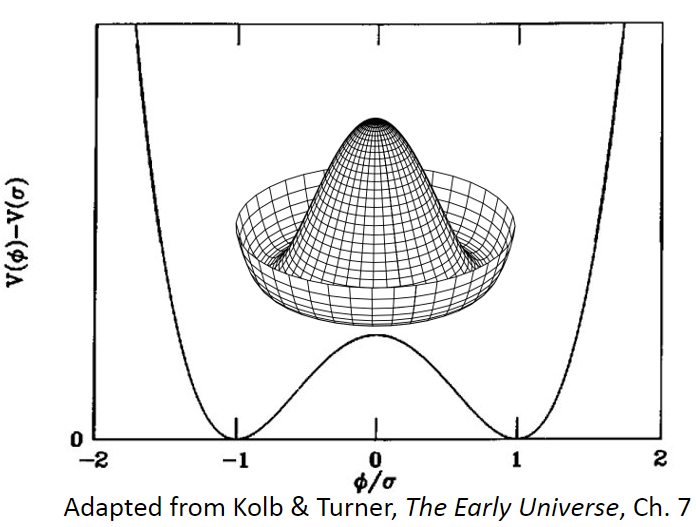
\includegraphics[width=250px]{Knipsel.PNG}    
\end{center}

I also added the 3-dimensional version, which most of us recognise as the Mexican hat graph.
We immediately recognise that the 2-dimensional graph has the following symmetry $\phi\mapsto -\phi$.
Which we also recognise in our Hamiltonian.
For the 3 dimensional version, the symmetry is $U(1)$.
In the 2 dimensional graph, we see that there are two minima. 
These are the two degenerate ground states.

Now we see that during the condensation of a state it reaches an unstable point in $\phi=0$.
Thus when it "falls" of this unstable point, there are two possibilities of ground states.
Due to quantum fluctuations and external factors, we cannot have the intermediate unstable state.
For conceptual reasons I have also included this picture which uses a rolling ball to show how the symmetry spontaneously breaks.

\begin{center}
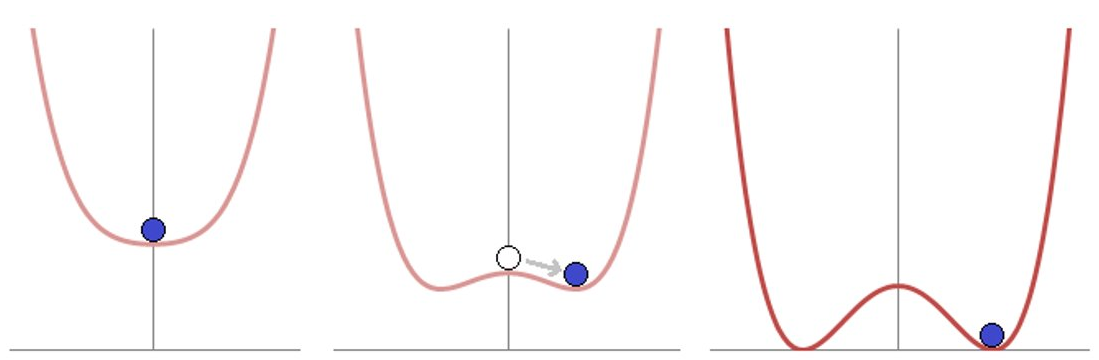
\includegraphics[width=350px]{Knipsel3.PNG}    
\end{center}


Spontaneous symmetry breaking is a concept in physics that is extremely useful and happens in a wide arrange of systems.
From cooling water to magnets, to the chirality of amino acids, to donkeys with multiple equally attractive hay bales.


%%% 894 words until here (including abstract)
%%% Maybe we have to delete temperature restoration! 



\subsection{High temperature restoration}

Until now we considered our field theory to live in a zero-temperature environment.
This couldn't be further from the truth in the early universe.
We already commented in the introduction that the early universe was an extreme place of temperatures that we can barely mimic by colliding protons at 99.999 996 4\% speed of light in the LHC.
Thus we must look at how such large temperatures affect the math.
We start by considering a heat bath where the theory lives in.
Therefore some of the math has to change slightly to account for this.
Namely we have to use an ensemble to calculate our partition function involving $\beta=\frac{1}{k_bT}$.
This has the direct consequence for the 2-point function $D_\beta$.

$$D_\beta (x-y)=\frac{\text{Tr} e^{-\beta H}\mathcal{T}[\phi(x)\phi(y)]}{\text{Tr} e^{-\beta H}}$$

It's clear that this two-point function heavily relies on the temperature.
The two-point function gives rise to loops that have to be renormalised and accounted for in the lagrangian.
Using the two-point function for calculating the one-loop correction for the potential you'll find.

\begin{center}
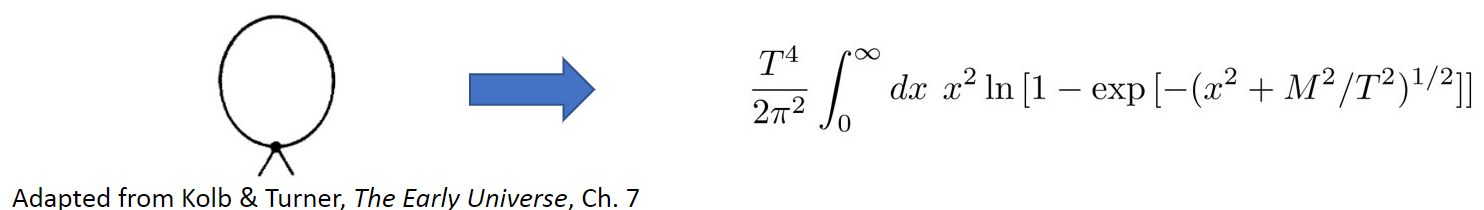
\includegraphics[width=450px]{Knipsel4.PNG}    
\end{center}

Now we have a corrected term for the effective potential, $V_T(\phi)=V(\phi)+\text{corrections}$.
First, let us, Taylor to high temperature the previous one-loop correction.
We find for the effective potential $V_T(\phi)$,
% show more of the Taylor expansion (straightforwardly from the book)

\begin{equation}
    V_T(\phi)=V(\phi)+\frac{\lambda}{8}T^2\phi^2-\frac{\pi}{90}T^4+\dots
\end{equation}

With $V(\phi)$ the potential of the $\phi-4$ model.
We can see that the temperature affects the graph in the parabolic part.
Let us also define the critical temperature $T_c$. 
Which is the temperature when the symmetry in the ground state is restored.
I have plotted 4 graphs.


\begin{center}
    
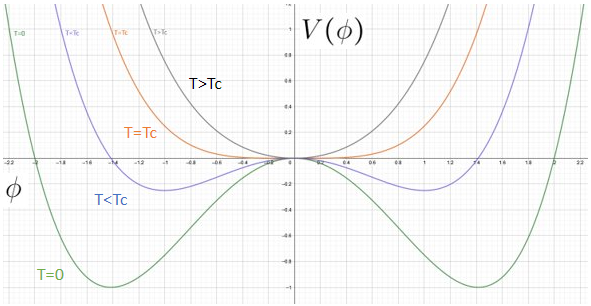
\includegraphics[]{graphTrestoration.PNG}

\end{center}

We start at a symmetry broken system in $T=0$. In $T>0$ case we start increasing the temperature, which results in rising of the two minima.
These minima vanish at $T=T_c$.
Where we immediately can see that the ground state will find itself in 0, which does have the symmetry of the Hamiltonian.
Temperatures greater than $T_c$ will not change much of the physics. 
Only the mass of the particle becomes greater.


%%% 1206 words until here (including abstract)



\section{Electroweak Symmetry breaking in the early universe}

In this section, we review the electroweak part of the standard model. We will see how the temperature dependence in the one loop corrected effective potential cause a second order phase transition. \\
\hspace{1cm}
The standard model is a so far quite successful quantum field theory that describes the elementary particles in our universe. 
The particles and therefore the fields involved can be classified as fermions $\psi^{i}$, gauge bosons $B, \,W^{a}_{a = 1\dots 3}, \, G^j_{j = 1\dots 8}$ and the Higgs boson $\Phi$. 

The fermions are described by spinors, the gauge bosons take values in the Lie algebra (i.e. they basically assign a matrix to every point in spacetime) and the Higgs boson is described by a spacetime depended complex  tuple. \\
The theory can be expressed in terms of its Lagrangian density $\mathcal{L}[\psi^{i}, B, W^{a}, G^{j}, \Psi]$. This Lagrangian density enjoys a $SU(3) \times SU(2) \times U(1)$ gauge symmetry. 
That means that at every point in spacetime, we can transform  all the fields differently by this gauge group and the Lagrangian density stays the same. Of course the transformation behaviour of the fields are crucial for the theory. The subgroup $SU(2)\times U(1)$ is called the \textit{electroweak symmetry} group. In particular, in the theory of the standard model, it is possible to perform a transformation of the electroweak symmetry group such that the Higgs field $\Phi$ gets reduced to a real scalar field. This is possible, because we can use the spacetime depended transformations to transform the complex two component vector of the Higgs field in every into 
\begin{align*}
    \Phi = \begin{pmatrix} 0 \\ \phi\end{pmatrix}, 
\end{align*}
where $\phi(x)$ is a real scalar field. We are left with a subgroup $U(1)$ of $SU(2) \times U(1)$. 
In order to keep this property in the theory, we must relinquish to do further electroweak symmetry transformations. So the theory with a real Higgs field remains with a $SU(3) \times U(1)$ symmetry. This partial choice of the gauge symmetry is called \textit{electroweak symmetry breaking}. \\
After the electroweak symmetry breaking, the Higgsboson appears in the Lagrangian density with the terms%https://www.overleaf.com/project/617baddb008ab998973df27a
\begin{align}
    \mathcal{L}_H[B, W, \psi^{i}, \phi] = -\frac{1}{2}(\partial_{\mu} \phi)^2 -\underbrace{\frac{g^2\phi^2}{8 \cos(\theta_{W})^2} Z_{\mu}^2-\frac{g^2 \phi^2}{8}|W_{\mu}|^2 }_{=\mathcal{L}_b } - \underbrace{\sum_{i}G_i\psi^{i}_R \phi \psi^{i}_L}_{=\mathcal{L}_{\psi}}+\underbrace{\frac{m^2}{2}\phi^2-\frac{\lambda}{4}\phi^4}_{ = V(\phi)} ,
    \label{eq:standardmodelLagrangianforHiggs}
\end{align}
where we defined the fields $Z_{\mu}  = -\sin(\theta_W)B_{\mu} + \cos(\theta_W)W^{3}_{\mu}$ and $W_{\mu} = (W^1_{\mu})^2 + (W^2_{\mu})^2$. The angle $\theta_W$ is called the Weinberg angle. The potential $V_{\phi}(\phi)$ is already familiar from equation $\eqref{eq:phi-4-Lagrangian}$. If we vary the Higgsfield $\phi$ in the Lagrangian \eqref{eq:standardmodelLagrangianforHiggs} around the minimum of the Higgs potential $V_{\phi}$, we see that gauge bosonic part $\mathcal{L}_{b}$ and the fermionic part $\mathcal{L}_{\psi}$ in the Lagrangian have mass terms depending on the minimum of the Higgs potential. This is how the mass terms for the fermions and bosons arise. \\
Therefore, we are much interested in the effective minimum of the potential for the Higgsfield $\phi$. But it is not sufficient to look at the minimum of $V_{\phi}$ but we want to consider the quantum corrections of one loops as well. In order to compute this, we can neglect the fermion couplings except for the coupling with the top quark, because the coupling of the top quark is so strong that it dominates the contribution for the fermions. 
With these corrections, the one loop effective potential reads
\begin{align*}
    V_{\phi}^{1loop}(\phi) =& -\frac{1}{2}m^2\phi + \frac{1}{4}\lambda\phi^4\\
    & +\frac{1}{64\pi^2}(-m^2 +3\lambda\phi^2)^2\ln\left(\frac{-m^2+3\lambda\phi^2}{\mu^2}\right)\\
    &+\frac{3}{1024 \pi^2}((2 + \frac{1}{\cos(\theta_W)^4})g^4)\phi^4 \ln\left(\frac{\phi^2}{\mu^2}\right)\\
    &-\frac{3}{64 \pi^2}G_t^4 \phi^4 \ln\left(\frac{\phi^2}{\mu^2}\right). 
\end{align*}

%J
Up to this point, we have considered the zero temperature one-loop effective potential, but we should also incorporate the temperature corrections because they played a primary role in the development of the phase transition in the early universe.
\\
It can be shown that temperature correction can be written as a sum of integrals of the form
\begin{equation}
F_{\pm}\left[X\left(\phi_{c}\right)\right] = \pm \int_{0}^{\infty} d x \quad x^{2} \ln \left[1 \mp \exp \left[-\left(x^{2}+\frac{X\left(\phi_{c}\right)}{ T^{2}}\right)^{1 / 2}\right]\right]
\end{equation}
where $F_+$ applies to boson loops and $F_-$ applies to fermion loops. Then, applying it to the one-loop effective potential we get
\begin{align*}
V_{T}\left(\phi_{c}\right)=V\left(\phi_{c}\right)+\frac{T^{4}}{2 \pi^{2}}&\left\{6 F_{+}\left[g^{2} \phi_{c}^{2} / 4\right]+3 F_{+}\left[\left(g^{2}+g^{\prime 2}\right) \phi_{c}^{2} / 4\right]\right. \\
&\left.+F_{+}\left[M^{2}\left(\phi_{c}\right)\right]+12 F_{-}\left[h_{t}^{2} \phi_{c}^{2} / 2\right]\right\}
\end{align*}
Although it is a complex expression, for what concerns us we can abstract the $F_{\pm}$ integrals away into a function such that
\begin{equation}
V_{T}\left(\phi_{c}\right)=V_{1 L}\left(\phi_{c}\right)+T^{4} \mathcal{F}\left(T, \phi_{c}, M_{H}, h_{t}, \ldots\right)
\end{equation}


This $T^4$ interaction recovers a first or second order electroweak phase transition through the aforementioned high temperature restoration. The final nature of the transition will depend on the value of the Higgs mass, and the specifics can be computed by taking the appropiate limits of $V_T$.

For the experimental value of the Higgs, we know that the transition must be second order because of (...).

Thus, unfortunately this disregards the possibility of a future experimental confirmation in the form of observing bubble nucleation.

%182 words


\section{First order phase transitions in Cosmology}
In the previous discussion we discovered that the electroweak phase transition in the early universe was a second-order phase transition.
It is also known, but not discussed in the presentation that the earlier phase transition associated with the strong force also was a second-order
phase transition. This leads to a problem: second-order phase transitions are smooth transitions, and no large energetic effects such as bubble 
nucleation are associated with these transitions. But this also leads to an opportunity: detecting any signals of a first-order phase transition 
cosmological data will point to physics beyond the current Standard Model

\section{Conclusion} %283 words
In this article we have made a concise outline of the most important points relevant to the electroweak phase transition that occurred in the early universe when the extreme temperatures of this cosmic period, averaging $T = xxK$ dropped below a critical value of $T_c=yyK$.

It has been essential to point out that this phase transition is caused by spontaneous symmetry breaking, in particular due to the instability of the vacuum state symmetric under $SU(2)_L \otimes U(1)_Y$ type gauge transformations. The fact that the non-symmetric vacuum has a lower energy drives the phase transition.

To do this, we have had to take a close look at the expression for the Higgs potential, considering both one-loop quantum corrections as well as temperature corrections. This latter term has played a key role in enabling high temperature symmetry restoration without which it is not possible to explain the cosmic phase transition.

We have also discussed how, in a generic way, phase transitions can be classified as first or second order, which gives rise to completely different physics. Second-order transitions are continuous, while first-order transitions exhibit a discontinuity that results in the release of latent energy. 

Cosmically, this distinction is of fundamental phenomenological importance since second order transitions are experimentally invisible, while the latent energy release for first order transitions is given in the form of nucleation bubbles, which propagate at the speed of light and leave a trace in the fabric of spacetime in the form of gravitational waves. We also concluded that this distinction is fundamentally given by the mass of the Higgs boson, and how a mass higher than $100$ GeV (as it occurs experimentally in reality, at $125$ GeV) gives rise to second-order transitions.


\end{document}
